
%% bare_adv.tex
%% V1.4b
%% 2015/08/26
%% by Michael Shell
%% See: 
%% http://www.michaelshell.org/
%% for current contact information.
%%
%% This is a skeleton file demonstrating the advanced use of IEEEtran.cls
%% (requires IEEEtran.cls version 1.8b or later) with an IEEE Computer
%% Society journal paper.
%%
%% Support sites:
%% http://www.michaelshell.org/tex/ieeetran/
%% http://www.ctan.org/pkg/ieeetran
%% and
%% http://www.ieee.org/

%%*************************************************************************
%% Legal Notice:
%% This code is offered as-is without any warranty either expressed or
%% implied; without even the implied warranty of MERCHANTABILITY or
%% FITNESS FOR A PARTICULAR PURPOSE! 
%% User assumes all risk.
%% In no event shall the IEEE or any contributor to this code be liable for
%% any damages or losses, including, but not limited to, incidental,
%% consequential, or any other damages, resulting from the use or misuse
%% of any information contained here.
%%
%% All comments are the opinions of their respective authors and are not
%% necessarily endorsed by the IEEE.
%%
%% This work is distributed under the LaTeX Project Public License (LPPL)
%% ( http://www.latex-project.org/ ) version 1.3, and may be freely used,
%% distributed and modified. A copy of the LPPL, version 1.3, is included
%% in the base LaTeX documentation of all distributions of LaTeX released
%% 2003/12/01 or later.
%% Retain all contribution notices and credits.
%% ** Modified files should be clearly indicated as such, including  **
%% ** renaming them and changing author support contact information. **
%%*************************************************************************


% *** Authors should verify (and, if needed, correct) their LaTeX system  ***
% *** with the testflow diagnostic prior to trusting their LaTeX platform ***
% *** with production work. The IEEE's font choices and paper sizes can   ***
% *** trigger bugs that do not appear when using other class files.       ***                          ***
% The testflow support page is at:
% http://www.michaelshell.org/tex/testflow/


% IEEEtran V1.7 and later provides for these CLASSINPUT macros to allow the
% user to reprogram some IEEEtran.cls defaults if needed. These settings
% override the internal defaults of IEEEtran.cls regardless of which class
% options are used. Do not use these unless you have good reason to do so as
% they can result in nonIEEE compliant documents. User beware. ;)
%
%\newcommand{\CLASSINPUTbaselinestretch}{1.0} % baselinestretch
%\newcommand{\CLASSINPUTinnersidemargin}{1in} % inner side margin
%\newcommand{\CLASSINPUToutersidemargin}{1in} % outer side margin
%\newcommand{\CLASSINPUTtoptextmargin}{1in}   % top text margin
%\newcommand{\CLASSINPUTbottomtextmargin}{1in}% bottom text margin




%
\documentclass[10pt,journal,compsoc]{IEEEtran}
% If IEEEtran.cls has not been installed into the LaTeX system files,
% manually specify the path to it like:
% \documentclass[10pt,journal,compsoc]{../sty/IEEEtran}


% For Computer Society journals, IEEEtran defaults to the use of 
% Palatino/Palladio as is done in IEEE Computer Society journals.
% To go back to Times Roman, you can use this code:
%\renewcommand{\rmdefault}{ptm}\selectfont





% Some very useful LaTeX packages include:
% (uncomment the ones you want to load)



% *** MISC UTILITY PACKAGES ***
%
%\usepackage{ifpdf}
% Heiko Oberdiek's ifpdf.sty is very useful if you need conditional
% compilation based on whether the output is pdf or dvi.
% usage:
% \ifpdf
%   % pdf code
% \else
%   % dvi code
% \fi
% The latest version of ifpdf.sty can be obtained from:
% http://www.ctan.org/pkg/ifpdf
% Also, note that IEEEtran.cls V1.7 and later provides a builtin
% \ifCLASSINFOpdf conditional that works the same way.
% When switching from latex to pdflatex and vice-versa, the compiler may
% have to be run twice to clear warning/error messages.






% *** CITATION PACKAGES ***
%
\ifCLASSOPTIONcompsoc
  % The IEEE Computer Society needs nocompress option
  % requires cite.sty v4.0 or later (November 2003)
  \usepackage[nocompress]{cite}
\else
  % normal IEEE
  \usepackage{cite}
\fi
% cite.sty was written by Donald Arseneau
% V1.6 and later of IEEEtran pre-defines the format of the cite.sty package
% \cite{} output to follow that of the IEEE. Loading the cite package will
% result in citation numbers being automatically sorted and properly
% "compressed/ranged". e.g., [1], [9], [2], [7], [5], [6] without using
% cite.sty will become [1], [2], [5]--[7], [9] using cite.sty. cite.sty's
% \cite will automatically add leading space, if needed. Use cite.sty's
% noadjust option (cite.sty V3.8 and later) if you want to turn this off
% such as if a citation ever needs to be enclosed in parenthesis.
% cite.sty is already installed on most LaTeX systems. Be sure and use
% version 5.0 (2009-03-20) and later if using hyperref.sty.
% The latest version can be obtained at:
% http://www.ctan.org/pkg/cite
% The documentation is contained in the cite.sty file itself.
%
% Note that some packages require special options to format as the Computer
% Society requires. In particular, Computer Society  papers do not use
% compressed citation ranges as is done in typical IEEE papers
% (e.g., [1]-[4]). Instead, they list every citation separately in order
% (e.g., [1], [2], [3], [4]). To get the latter we need to load the cite
% package with the nocompress option which is supported by cite.sty v4.0
% and later.





% *** GRAPHICS RELATED PACKAGES ***
%
\ifCLASSINFOpdf
  \usepackage[pdftex]{graphicx}
  
  % declare the path(s) where your graphic files are
  % \graphicspath{{../pdf/}{../jpeg/}}
  % and their extensions so you won't have to specify these with
  % every instance of \includegraphics
  % \DeclareGraphicsExtensions{.pdf,.jpeg,.png}
\else
  % or other class option (dvipsone, dvipdf, if not using dvips). graphicx
  % will default to the driver specified in the system graphics.cfg if no
  % driver is specified.
  % \usepackage[dvips]{graphicx}
  % declare the path(s) where your graphic files are
  % \graphicspath{{../eps/}}
  % and their extensions so you won't have to specify these with
  % every instance of \includegraphics
  % \DeclareGraphicsExtensions{.eps}
\fi
% graphicx was written by David Carlisle and Sebastian Rahtz. It is
% required if you want graphics, photos, etc. graphicx.sty is already
% installed on most LaTeX systems. The latest version and documentation
% can be obtained at: 
% http://www.ctan.org/pkg/graphicx
% Another good source of documentation is "Using Imported Graphics in
% LaTeX2e" by Keith Reckdahl which can be found at:
% http://www.ctan.org/pkg/epslatex
%
% latex, and pdflatex in dvi mode, support graphics in encapsulated
% postscript (.eps) format. pdflatex in pdf mode supports graphics
% in .pdf, .jpeg, .png and .mps (metapost) formats. Users should ensure
% that all non-photo figures use a vector format (.eps, .pdf, .mps) and
% not a bitmapped formats (.jpeg, .png). The IEEE frowns on bitmapped formats
% which can result in "jaggedy"/blurry rendering of lines and letters as
% well as large increases in file sizes.
%
% You can find documentation about the pdfTeX application at:
% http://www.tug.org/applications/pdftex





% *** MATH PACKAGES ***
%
\usepackage{amsmath}
% A popular package from the American Mathematical Society that provides
% many useful and powerful commands for dealing with mathematics.
%
% Note that the amsmath package sets \interdisplaylinepenalty to 10000
% thus preventing page breaks from occurring within multiline equations. Use:
%\interdisplaylinepenalty=2500
% after loading amsmath to restore such page breaks as IEEEtran.cls normally
% does. amsmath.sty is already installed on most LaTeX systems. The latest
% version and documentation can be obtained at:
% http://www.ctan.org/pkg/amsmath





% *** SPECIALIZED LIST PACKAGES ***
%\usepackage{acronym}
% acronym.sty was written by Tobias Oetiker. This package provides tools for
% managing documents with large numbers of acronyms. (You don't *have* to
% use this package - unless you have a lot of acronyms, you may feel that
% such package management of them is bit of an overkill.)
% Do note that the acronym environment (which lists acronyms) will have a
% problem when used under IEEEtran.cls because acronym.sty relies on the
% description list environment - which IEEEtran.cls has customized for
% producing IEEE style lists. A workaround is to declared the longest
% label width via the IEEEtran.cls \IEEEiedlistdecl global control:
%
% \renewcommand{\IEEEiedlistdecl}{\IEEEsetlabelwidth{SONET}}
% \begin{acronym}
%
% \end{acronym}
% \renewcommand{\IEEEiedlistdecl}{\relax}% remember to reset \IEEEiedlistdecl
%
% instead of using the acronym environment's optional argument.
% The latest version and documentation can be obtained at:
% http://www.ctan.org/pkg/acronym


%\usepackage{algorithmic}
% algorithmic.sty was written by Peter Williams and Rogerio Brito.
% This package provides an algorithmic environment fo describing algorithms.
% You can use the algorithmic environment in-text or within a figure
% environment to provide for a floating algorithm. Do NOT use the algorithm
% floating environment provided by algorithm.sty (by the same authors) or
% algorithm2e.sty (by Christophe Fiorio) as the IEEE does not use dedicated
% algorithm float types and packages that provide these will not provide
% correct IEEE style captions. The latest version and documentation of
% algorithmic.sty can be obtained at:
% http://www.ctan.org/pkg/algorithms
% Also of interest may be the (relatively newer and more customizable)
% algorithmicx.sty package by Szasz Janos:
% http://www.ctan.org/pkg/algorithmicx




% *** ALIGNMENT PACKAGES ***
%
%\usepackage{array}
% Frank Mittelbach's and David Carlisle's array.sty patches and improves
% the standard LaTeX2e array and tabular environments to provide better
% appearance and additional user controls. As the default LaTeX2e table
% generation code is lacking to the point of almost being broken with
% respect to the quality of the end results, all users are strongly
% advised to use an enhanced (at the very least that provided by array.sty)
% set of table tools. array.sty is already installed on most systems. The
% latest version and documentation can be obtained at:
% http://www.ctan.org/pkg/array


%\usepackage{mdwmath}
%\usepackage{mdwtab}
% Also highly recommended is Mark Wooding's extremely powerful MDW tools,
% especially mdwmath.sty and mdwtab.sty which are used to format equations
% and tables, respectively. The MDWtools set is already installed on most
% LaTeX systems. The lastest version and documentation is available at:
% http://www.ctan.org/pkg/mdwtools


% IEEEtran contains the IEEEeqnarray family of commands that can be used to
% generate multiline equations as well as matrices, tables, etc., of high
% quality.


%\usepackage{eqparbox}
% Also of notable interest is Scott Pakin's eqparbox package for creating
% (automatically sized) equal width boxes - aka "natural width parboxes".
% Available at:
% http://www.ctan.org/pkg/eqparbox




% *** SUBFIGURE PACKAGES ***
%\ifCLASSOPTIONcompsoc
%  \usepackage[caption=false,font=footnotesize,labelfont=sf,textfont=sf]{subfig}
%\else
%  \usepackage[caption=false,font=footnotesize]{subfig}
%\fi
% subfig.sty, written by Steven Douglas Cochran, is the modern replacement
% for subfigure.sty, the latter of which is no longer maintained and is
% incompatible with some LaTeX packages including fixltx2e. However,
% subfig.sty requires and automatically loads Axel Sommerfeldt's caption.sty
% which will override IEEEtran.cls' handling of captions and this will result
% in non-IEEE style figure/table captions. To prevent this problem, be sure
% and invoke subfig.sty's "caption=false" package option (available since
% subfig.sty version 1.3, 2005/06/28) as this is will preserve IEEEtran.cls
% handling of captions.
% Note that the Computer Society format requires a sans serif font rather
% than the serif font used in traditional IEEE formatting and thus the need
% to invoke different subfig.sty package options depending on whether
% compsoc mode has been enabled.
%
% The latest version and documentation of subfig.sty can be obtained at:
% http://www.ctan.org/pkg/subfig




% *** FLOAT PACKAGES ***
%
%\usepackage{fixltx2e}
% fixltx2e, the successor to the earlier fix2col.sty, was written by
% Frank Mittelbach and David Carlisle. This package corrects a few problems
% in the LaTeX2e kernel, the most notable of which is that in current
% LaTeX2e releases, the ordering of single and double column floats is not
% guaranteed to be preserved. Thus, an unpatched LaTeX2e can allow a
% single column figure to be placed prior to an earlier double column
% figure.
% Be aware that LaTeX2e kernels dated 2015 and later have fixltx2e.sty's
% corrections already built into the system in which case a warning will
% be issued if an attempt is made to load fixltx2e.sty as it is no longer
% needed.
% The latest version and documentation can be found at:
% http://www.ctan.org/pkg/fixltx2e


\usepackage{stfloats}
% stfloats.sty was written by Sigitas Tolusis. This package gives LaTeX2e
% the ability to do double column floats at the bottom of the page as well
% as the top. (e.g., "\begin{figure*}[!b]" is not normally possible in
% LaTeX2e). It also provides a command:
%\fnbelowfloat
% to enable the placement of footnotes below bottom floats (the standard
% LaTeX2e kernel puts them above bottom floats). This is an invasive package
% which rewrites many portions of the LaTeX2e float routines. It may not work
% with other packages that modify the LaTeX2e float routines. The latest
% version and documentation can be obtained at:
% http://www.ctan.org/pkg/stfloats
% Do not use the stfloats baselinefloat ability as the IEEE does not allow
% \baselineskip to stretch. Authors submitting work to the IEEE should note
% that the IEEE rarely uses double column equations and that authors should try
% to avoid such use. Do not be tempted to use the cuted.sty or midfloat.sty
% packages (also by Sigitas Tolusis) as the IEEE does not format its papers in
% such ways.
% Do not attempt to use stfloats with fixltx2e as they are incompatible.
% Instead, use Morten Hogholm'a dblfloatfix which combines the features
% of both fixltx2e and stfloats:
%
% \usepackage{dblfloatfix}
% The latest version can be found at:
% http://www.ctan.org/pkg/dblfloatfix


%\ifCLASSOPTIONcaptionsoff
%  \usepackage[nomarkers]{endfloat}
% \let\MYoriglatexcaption\caption
% \renewcommand{\caption}[2][\relax]{\MYoriglatexcaption[#2]{#2}}
%\fi
% endfloat.sty was written by James Darrell McCauley, Jeff Goldberg and 
% Axel Sommerfeldt. This package may be useful when used in conjunction with 
% IEEEtran.cls'  captionsoff option. Some IEEE journals/societies require that
% submissions have lists of figures/tables at the end of the paper and that
% figures/tables without any captions are placed on a page by themselves at
% the end of the document. If needed, the draftcls IEEEtran class option or
% \CLASSINPUTbaselinestretch interface can be used to increase the line
% spacing as well. Be sure and use the nomarkers option of endfloat to
% prevent endfloat from "marking" where the figures would have been placed
% in the text. The two hack lines of code above are a slight modification of
% that suggested by in the endfloat docs (section 8.4.1) to ensure that
% the full captions always appear in the list of figures/tables - even if
% the user used the short optional argument of \caption[]{}.
% IEEE papers do not typically make use of \caption[]'s optional argument,
% so this should not be an issue. A similar trick can be used to disable
% captions of packages such as subfig.sty that lack options to turn off
% the subcaptions:
% For subfig.sty:
% \let\MYorigsubfloat\subfloat
% \renewcommand{\subfloat}[2][\relax]{\MYorigsubfloat[]{#2}}
% However, the above trick will not work if both optional arguments of
% the \subfloat command are used. Furthermore, there needs to be a
% description of each subfigure *somewhere* and endfloat does not add
% subfigure captions to its list of figures. Thus, the best approach is to
% avoid the use of subfigure captions (many IEEE journals avoid them anyway)
% and instead reference/explain all the subfigures within the main caption.
% The latest version of endfloat.sty and its documentation can obtained at:
% http://www.ctan.org/pkg/endfloat
%
% The IEEEtran \ifCLASSOPTIONcaptionsoff conditional can also be used
% later in the document, say, to conditionally put the References on a 
% page by themselves.





% *** PDF, URL AND HYPERLINK PACKAGES ***
%
%\usepackage{url}
% url.sty was written by Donald Arseneau. It provides better support for
% handling and breaking URLs. url.sty is already installed on most LaTeX
% systems. The latest version and documentation can be obtained at:
% http://www.ctan.org/pkg/url
% Basically, \url{my_url_here}.


% NOTE: PDF thumbnail features are not required in IEEE papers
%       and their use requires extra complexity and work.
%\ifCLASSINFOpdf
%  \usepackage[pdftex]{thumbpdf}
%\else
%  \usepackage[dvips]{thumbpdf}
%\fi
% thumbpdf.sty and its companion Perl utility were written by Heiko Oberdiek.
% It allows the user a way to produce PDF documents that contain fancy
% thumbnail images of each of the pages (which tools like acrobat reader can
% utilize). This is possible even when using dvi->ps->pdf workflow if the
% correct thumbpdf driver options are used. thumbpdf.sty incorporates the
% file containing the PDF thumbnail information (filename.tpm is used with
% dvips, filename.tpt is used with pdftex, where filename is the base name of
% your tex document) into the final ps or pdf output document. An external
% utility, the thumbpdf *Perl script* is needed to make these .tpm or .tpt
% thumbnail files from a .ps or .pdf version of the document (which obviously
% does not yet contain pdf thumbnails). Thus, one does a:
% 
% thumbpdf filename.pdf 
%
% to make a filename.tpt, and:
%
% thumbpdf --mode dvips filename.ps
%
% to make a filename.tpm which will then be loaded into the document by
% thumbpdf.sty the NEXT time the document is compiled (by pdflatex or
% latex->dvips->ps2pdf). Users must be careful to regenerate the .tpt and/or
% .tpm files if the main document changes and then to recompile the
% document to incorporate the revised thumbnails to ensure that thumbnails
% match the actual pages. It is easy to forget to do this!
% 
% Unix systems come with a Perl interpreter. However, MS Windows users
% will usually have to install a Perl interpreter so that the thumbpdf
% script can be run. The Ghostscript PS/PDF interpreter is also required.
% See the thumbpdf docs for details. The latest version and documentation
% can be obtained at.
% http://www.ctan.org/pkg/thumbpdf


% NOTE: PDF hyperlink and bookmark features are not required in IEEE
%       papers and their use requires extra complexity and work.
% *** IF USING HYPERREF BE SURE AND CHANGE THE EXAMPLE PDF ***
% *** TITLE/SUBJECT/AUTHOR/KEYWORDS INFO BELOW!!           ***
\newcommand\MYhyperrefoptions{bookmarks=true,bookmarksnumbered=true,
pdfpagemode={UseOutlines},plainpages=false,pdfpagelabels=true,
colorlinks=true,linkcolor={black},citecolor={black},urlcolor={black},
pdftitle={Bare Demo of IEEEtran.cls for Computer Society Journals},%<!CHANGE!
pdfsubject={Typesetting},%<!CHANGE!
pdfauthor={Michael D. Shell},%<!CHANGE!
pdfkeywords={Computer Society, IEEEtran, journal, LaTeX, paper,
             template}}%<^!CHANGE!
%\ifCLASSINFOpdf
%\usepackage[\MYhyperrefoptions,pdftex]{hyperref}
%\else
%\usepackage[\MYhyperrefoptions,breaklinks=true,dvips]{hyperref}
%\usepackage{breakurl}
%\fi
% One significant drawback of using hyperref under DVI output is that the
% LaTeX compiler cannot break URLs across lines or pages as can be done
% under pdfLaTeX's PDF output via the hyperref pdftex driver. This is
% probably the single most important capability distinction between the
% DVI and PDF output. Perhaps surprisingly, all the other PDF features
% (PDF bookmarks, thumbnails, etc.) can be preserved in
% .tex->.dvi->.ps->.pdf workflow if the respective packages/scripts are
% loaded/invoked with the correct driver options (dvips, etc.). 
% As most IEEE papers use URLs sparingly (mainly in the references), this
% may not be as big an issue as with other publications.
%
% That said, Vilar Camara Neto created his breakurl.sty package which
% permits hyperref to easily break URLs even in dvi mode.
% Note that breakurl, unlike most other packages, must be loaded
% AFTER hyperref. The latest version of breakurl and its documentation can
% be obtained at:
% http://www.ctan.org/pkg/breakurl
% breakurl.sty is not for use under pdflatex pdf mode.
%
% The advanced features offer by hyperref.sty are not required for IEEE
% submission, so users should weigh these features against the added
% complexity of use.
% The package options above demonstrate how to enable PDF bookmarks
% (a type of table of contents viewable in Acrobat Reader) as well as
% PDF document information (title, subject, author and keywords) that is
% viewable in Acrobat reader's Document_Properties menu. PDF document
% information is also used extensively to automate the cataloging of PDF
% documents. The above set of options ensures that hyperlinks will not be
% colored in the text and thus will not be visible in the printed page,
% but will be active on "mouse over". USING COLORS OR OTHER HIGHLIGHTING
% OF HYPERLINKS CAN RESULT IN DOCUMENT REJECTION BY THE IEEE, especially if
% these appear on the "printed" page. IF IN DOUBT, ASK THE RELEVANT
% SUBMISSION EDITOR. You may need to add the option hypertexnames=false if
% you used duplicate equation numbers, etc., but this should not be needed
% in normal IEEE work.
% The latest version of hyperref and its documentation can be obtained at:
% http://www.ctan.org/pkg/hyperref


\usepackage{amssymb}


% *** Do not adjust lengths that control margins, column widths, etc. ***
% *** Do not use packages that alter fonts (such as pslatex).         ***
% There should be no need to do such things with IEEEtran.cls V1.6 and later.
% (Unless specifically asked to do so by the journal or conference you plan
% to submit to, of course. )


% correct bad hyphenation here
\hyphenation{op-tical net-works semi-conduc-tor}


\begin{document}
%
% paper title
% Titles are generally capitalized except for words such as a, an, and, as,
% at, but, by, for, in, nor, of, on, or, the, to and up, which are usually
% not capitalized unless they are the first or last word of the title.
% Linebreaks \\ can be used within to get better formatting as desired.
% Do not put math or special symbols in the title.
\title{Data Augmentation Powered by \\ Generative Adversarial Network}
%
%
% author names and IEEE memberships
% note positions of commas and nonbreaking spaces ( ~ ) LaTeX will not break
% a structure at a ~ so this keeps an author's name from being broken across
% two lines.
% use \thanks{} to gain access to the first footnote area
% a separate \thanks must be used for each paragraph as LaTeX2e's \thanks
% was not built to handle multiple paragraphs
%
%
%\IEEEcompsocitemizethanks is a special \thanks that produces the bulleted
% lists the Computer Society journals use for "first footnote" author
% affiliations. Use \IEEEcompsocthanksitem which works much like \item
% for each affiliation group. When not in compsoc mode,
% \IEEEcompsocitemizethanks becomes like \thanks and
% \IEEEcompsocthanksitem becomes a line break with idention. This
% facilitates dual compilation, although admittedly the differences in the
% desired content of \author between the different types of papers makes a
% one-size-fits-all approach a daunting prospect. For instance, compsoc 
% journal papers have the author affiliations above the "Manuscript
% received ..."  text while in non-compsoc journals this is reversed. Sigh.

\author{Szabolcs~Hornyák, Károly~Póka}

% note the % following the last \IEEEmembership and also \thanks - 
% these prevent an unwanted space from occurring between the last author name
% and the end of the author line. i.e., if you had this:
% 
% \author{....lastname \thanks{...} \thanks{...} }
%                     ^------------^------------^----Do not want these spaces!
%
% a space would be appended to the last name and could cause every name on that
% line to be shifted left slightly. This is one of those "LaTeX things". For
% instance, "\textbf{A} \textbf{B}" will typeset as "A B" not "AB". To get
% "AB" then you have to do: "\textbf{A}\textbf{B}"
% \thanks is no different in this regard, so shield the last } of each \thanks
% that ends a line with a % and do not let a space in before the next \thanks.
% Spaces after \IEEEmembership other than the last one are OK (and needed) as
% you are supposed to have spaces between the names. For what it is worth,
% this is a minor point as most people would not even notice if the said evil
% space somehow managed to creep in.



% The paper headers
%\markboth{Journal of \LaTeX\ Class Files,~Vol.~14, No.~8, August~2015}%
%{Shell \MakeLowercase{\textit{et al.}}: Bare Advanced Demo of IEEEtran.cls for IEEE Computer %Society Journals}
% The only time the second header will appear is for the odd numbered pages
% after the title page when using the twoside option.
% 
% *** Note that you probably will NOT want to include the author's ***
% *** name in the headers of peer review papers.                   ***
% You can use \ifCLASSOPTIONpeerreview for conditional compilation here if
% you desire.



% The publisher's ID mark at the bottom of the page is less important with
% Computer Society journal papers as those publications place the marks
% outside of the main text columns and, therefore, unlike regular IEEE
% journals, the available text space is not reduced by their presence.
% If you want to put a publisher's ID mark on the page you can do it like
% this:
%\IEEEpubid{0000--0000/00\$00.00~\copyright~2015 IEEE}
% or like this to get the Computer Society new two part style.
%\IEEEpubid{\makebox[\columnwidth]{\hfill 0000--0000/00/\$00.00~\copyright~2015 IEEE}%
%\hspace{\columnsep}\makebox[\columnwidth]{Published by the IEEE Computer Society\hfill}}
% Remember, if you use this you must call \IEEEpubidadjcol in the second
% column for its text to clear the IEEEpubid mark (Computer Society journal
% papers don't need this extra clearance.)



% use for special paper notices
%\IEEEspecialpapernotice{(Invited Paper)}



% for Computer Society papers, we must declare the abstract and index terms
% PRIOR to the title within the \IEEEtitleabstractindextext IEEEtran
% command as these need to go into the title area created by \maketitle.
% As a general rule, do not put math, special symbols or citations
% in the abstract or keywords.
\IEEEtitleabstractindextext{%
\begin{abstract}
Classical data augmentation techniques are not sufficient for facial recognition problems with small datasets. In this paper we present our work aimed to develop generative models for data augmentation. We studied several GANs that provide control over the features of the generated images, then tried to implement a model that can be used for altering attributes of real images. We experimented with multiple architectures, studied the effects of certain loss functions and the practical limits of image recovery. Our attempts moved towards the aforementioned goal but was not reached during the semester. At last we found but did not come to thoroughtly examine great methods to improve the quality of the generated images. We will continue to develop our solution with these methods and the experience gained from the project.
\end{abstract}

% Note that keywords are not normally used for peerreview papers.
\begin{IEEEkeywords}
Generative Adversarial Network, GAN, InfoGAN, BEGAN, data augmentation, facial recognition
\end{IEEEkeywords}}


% make the title area
\maketitle


% To allow for easy dual compilation without having to reenter the
% abstract/keywords data, the \IEEEtitleabstractindextext text will
% not be used in maketitle, but will appear (i.e., to be "transported")
% here as \IEEEdisplaynontitleabstractindextext when compsoc mode
% is not selected <OR> if conference mode is selected - because compsoc
% conference papers position the abstract like regular (non-compsoc)
% papers do!
\IEEEdisplaynontitleabstractindextext
% \IEEEdisplaynontitleabstractindextext has no effect when using
% compsoc under a non-conference mode.


% For peer review papers, you can put extra information on the cover
% page as needed:
% \ifCLASSOPTIONpeerreview
% \begin{center} \bfseries EDICS Category: 3-BBND \end{center}
% \fi
%
% For peerreview papers, this IEEEtran command inserts a page break and
% creates the second title. It will be ignored for other modes.
\IEEEpeerreviewmaketitle


\ifCLASSOPTIONcompsoc
\IEEEraisesectionheading{\section{Introduction}\label{sec:introduction}}
\else
\section{Introduction}
\label{sec:introduction}
\fi
% Computer Society journal (but not conference!) papers do something unusual
% with the very first section heading (almost always called "Introduction").
% They place it ABOVE the main text! IEEEtran.cls does not automatically do
% this for you, but you can achieve this effect with the provided
% \IEEEraisesectionheading{} command. Note the need to keep any \label that
% is to refer to the section immediately after \section in the above as
% \IEEEraisesectionheading puts \section within a raised box.




% The very first letter is a 2 line initial drop letter followed
% by the rest of the first word in caps (small caps for compsoc).
% 
% form to use if the first word consists of a single letter:
% \IEEEPARstart{A}{demo} file is ....
% 
% form to use if you need the single drop letter followed by
% normal text (unknown if ever used by the IEEE):
% \IEEEPARstart{A}{}demo file is ....
% 
% Some journals put the first two words in caps:
% \IEEEPARstart{T}{his demo} file is ....
% 
% Here we have the typical use of a "T" for an initial drop letter
% and "HIS" in caps to complete the first word.
\IEEEPARstart{F}{acial} recognition is a popular field  of deep learning nowadays. Numerous methods and network architectures has been developed and applications range from authentication and security to diagnosing certain medical conditions.

One of the main problem of deep learning applications is data shortage, and it is also frequent in facial recognition. For example to train a neural network to recognize the rightful owner of the car it is embedded into would require an impossible amount of image data from the driver. The problem can be addressed by use of transfer learning methods and/or data augmentation techniques. While transfer learning is a great way to exploit the capabilities of pretrained models, changes in facial attributes such as growing a beard or getting glasses would require the system to adapt by retraining itself. Use of data augmentation faces the same problem because its image transformations do not alter the features of the given image.

Our solution is aimed towards generative data augmentation to address the above mentioned problems. We examined and extended improved versions of the InfoGAN architecture to generate and regenerate high quality images and controlling their features in the latent space. This approach enables the original dataset to be augmented in a meaningful way, generating images of the same face with different features. Because components of the latent vector can be connected to facial attributes, data augmentation becomes the exploration of the latent space in different directions.

After the theoretical basis of generative networks we list the existing GAN architectures that provide control over image attributes. Then we describe our extensions and modifications made to these architectures and present the results.

% You must have at least 2 lines in the paragraph with the drop letter
% (should never be an issue)
 %\cite{abdal2019image2stylegan}

%\begin{figure}[h]
%	\centering
%	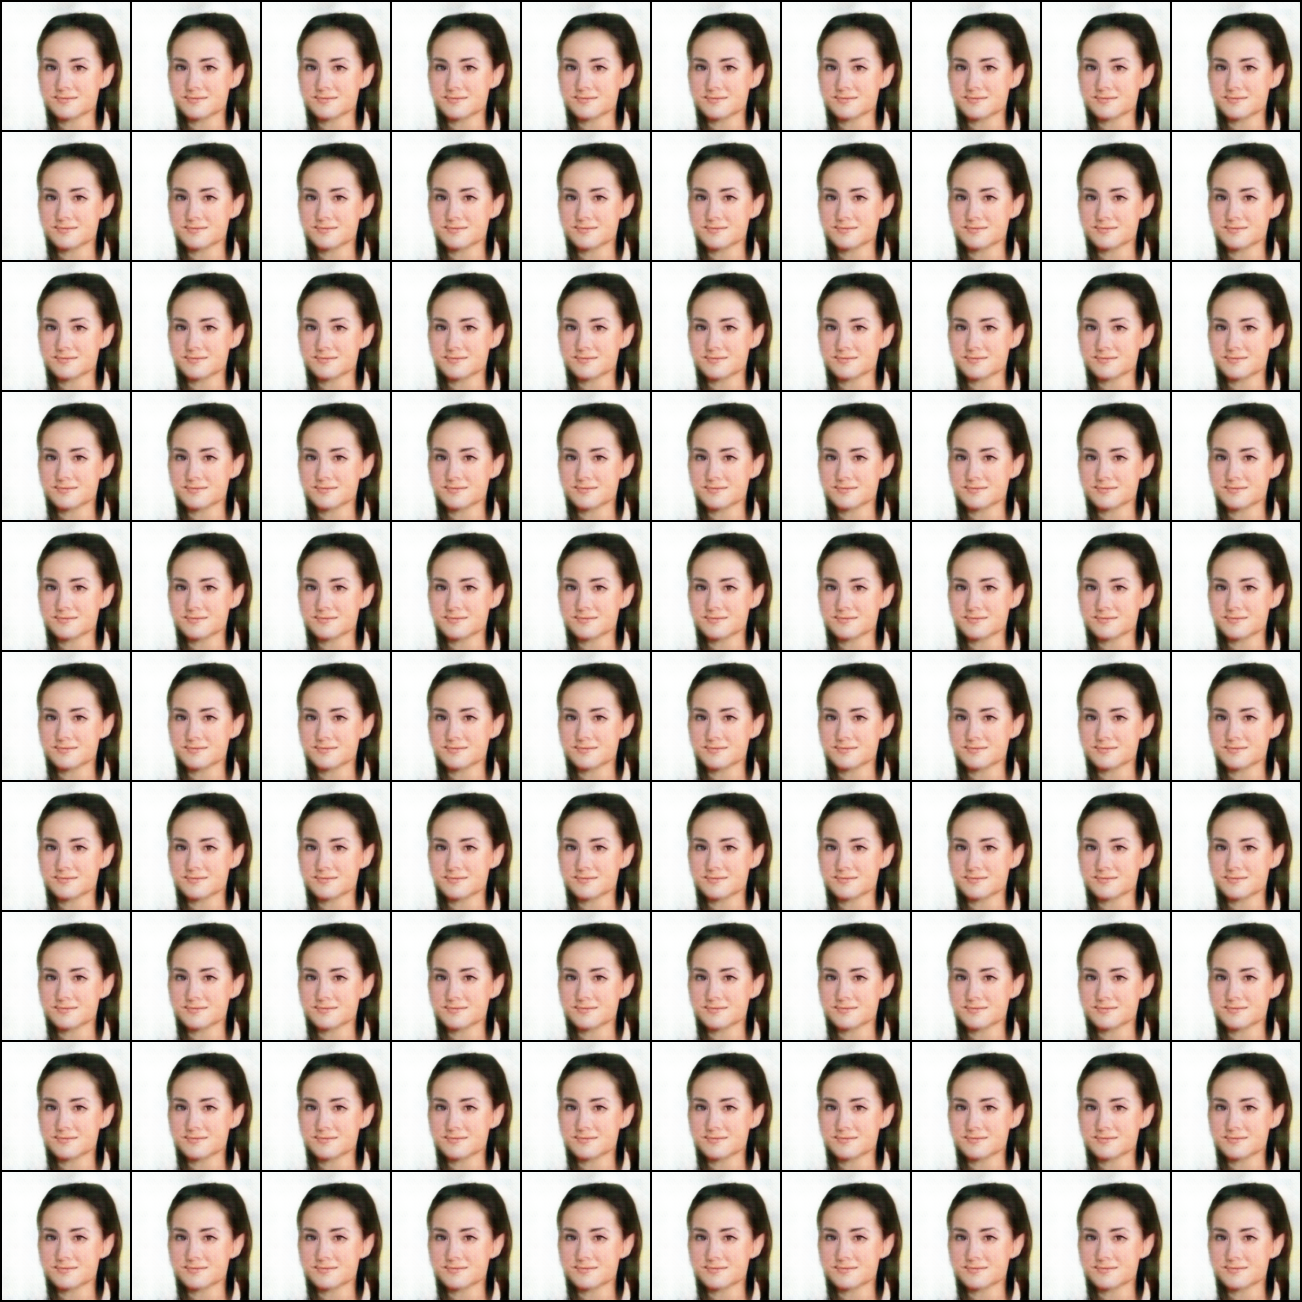
\includegraphics[width=1\linewidth]{girl_static_100}
%	\caption{Reconstructed image of a girl from CelebA}
%	\label{fig:girl_static}
%\end{figure}

%\hfill mds
 
%\hfill August 26, 2015

% An example of a floating figure using the graphicx package.
% Note that \label must occur AFTER (or within) \caption.
% For figures, \caption should occur after the \includegraphics.
% Note that IEEEtran v1.7 and later has special internal code that
% is designed to preserve the operation of \label within \caption
% even when the captionsoff option is in effect. However, because
% of issues like this, it may be the safest practice to put all your
% \label just after \caption rather than within \caption{}.
%
% Reminder: the "draftcls" or "draftclsnofoot", not "draft", class
% option should be used if it is desired that the figures are to be
% displayed while in draft mode.
%
%\begin{figure}[!t]
%\centering
%\includegraphics[width=2.5in]{myfigure}
% where an .eps filename suffix will be assumed under latex, 
% and a .pdf suffix will be assumed for pdflatex; or what has been declared
% via \DeclareGraphicsExtensions.
%\caption{Simulation results for the network.}
%\label{fig_sim}
%\end{figure}

% Note that the IEEE typically puts floats only at the top, even when this
% results in a large percentage of a column being occupied by floats.
% However, the Computer Society has been known to put floats at the bottom.


% An example of a double column floating figure using two subfigures.
% (The subfig.sty package must be loaded for this to work.)
% The subfigure \label commands are set within each subfloat command,
% and the \label for the overall figure must come after \caption.
% \hfil is used as a separator to get equal spacing.
% Watch out that the combined width of all the subfigures on a 
% line do not exceed the text width or a line break will occur.
%
%\begin{figure*}[!t]
%\centering
%\subfloat[Case I]{\includegraphics[width=2.5in]{box}%
%\label{fig_first_case}}
%\hfil
%\subfloat[Case II]{\includegraphics[width=2.5in]{box}%
%\label{fig_second_case}}
%\caption{Simulation results for the network.}
%\label{fig_sim}
%\end{figure*}
%
% Note that often IEEE papers with subfigures do not employ subfigure
% captions (using the optional argument to \subfloat[]), but instead will
% reference/describe all of them (a), (b), etc., within the main caption.
% Be aware that for subfig.sty to generate the (a), (b), etc., subfigure
% labels, the optional argument to \subfloat must be present. If a
% subcaption is not desired, just leave its contents blank,
% e.g., \subfloat[].


% An example of a floating table. Note that, for IEEE style tables, the
% \caption command should come BEFORE the table and, given that table
% captions serve much like titles, are usually capitalized except for words
% such as a, an, and, as, at, but, by, for, in, nor, of, on, or, the, to
% and up, which are usually not capitalized unless they are the first or
% last word of the caption. Table text will default to \footnotesize as
% the IEEE normally uses this smaller font for tables.
% The \label must come after \caption as always.
%
%\begin{table}[!t]
%% increase table row spacing, adjust to taste
%\renewcommand{\arraystretch}{1.3}
% if using array.sty, it might be a good idea to tweak the value of
% \extrarowheight as needed to properly center the text within the cells
%\caption{An Example of a Table}
%\label{table_example}
%\centering
%% Some packages, such as MDW tools, offer better commands for making tables
%% than the plain LaTeX2e tabular which is used here.
%\begin{tabular}{|c||c|}
%\hline
%One & Two\\
%\hline
%Three & Four\\
%\hline
%\end{tabular}
%\end{table}


% Note that the IEEE does not put floats in the very first column
% - or typically anywhere on the first page for that matter. Also,
% in-text middle ("here") positioning is typically not used, but it
% is allowed and encouraged for Computer Society conferences (but
% not Computer Society journals). Most IEEE journals/conferences use
% top floats exclusively. 
% Note that, LaTeX2e, unlike IEEE journals/conferences, places
% footnotes above bottom floats. This can be corrected via the
% \fnbelowfloat command of the stfloats package.




\section{Basic theory of GANs}
The abbreviation "GAN" stands for Generative Adversarial Network and it was published by Goodfellow et al. \cite{goodfellow2014generative} in 2014. It comprises of a generator and a discriminator network. These networks compete during training:

\begin{itemize}
	\item the objective of the discriminator is to distinguish between real and generated images,
	\item the objective of the generator is to fool the discriminator by generating images indistinguishable from real ones. 
\end{itemize}

These opposing objectives can be formulated as:

\begin{equation}
\begin{aligned}
	\min_G \max_D V(D,G) &= \mathbb{E}_{x\sim p_{data}(x)}\left[ \mathrm{log}D(x) \right] \\
	&+ \mathbb{E}_{z\sim p_{z}(z)}\left[ \mathrm{log}(1-D(G(z)))\right]
\end{aligned}
\end{equation}

During training we alternate between $k$ steps of optimizing the discriminator and one step of optimizing the generator network, where $k$ is a hyperparameter usually set to 1.

The GAN architecture provided much better results then previous methods. The downside of the "vanilla" GAN architecture is that the representation of image features in the latent space become highly entangled \cite{radford2015unsupervised}, hence any change made to the latent vector will effect multiple attributes of the generated image.

\section{CelebA dataset}

For the training of every model we used the Large-scale CelebFaces Attributes (CelebA) dataset. This set contains 202599 celebrity images, each with 40 attribute annotation but we only used the pure cropped images without annotation. CelebA has a large diversity and quantity. We can find faces with glasses, in various poses and with different mimics. The cropped size of the images is 178x218 which seems poor but the dilemma of the generation size can be easily a memory consuming problem.

\section{Experiments with existing architectures}

Because the basic architecture of GANs does not provide control over the features of the generated images we looked for more advanced architectures.

\subsection{InfoGAN}

The first network we examined was the InfoGAN by Chen et al. \cite{chen2016infogan} and some of its improved versions \cite{10.1007/978-3-319-78452-6_5}\cite{mirza2014conditional}. This generative architecture attempts to control the features of the generated images via so called code components concatenated to the latent (noise) vector. In order to encourage the generator to connect these code components to meaningful image features (to learn a disentangled representation) the authors introduced a new criteria in the generator's loss function: the generator should maximize the mutual information between the input latent vector and the generated image.

The total loss of the generator ($L_G$) is defined as:

\begin{equation}\label{g_loss}
	L_G = -L_D(x_G) - \lambda I([z,c], x_G)
\end{equation}
where $L_D(x_G)$ is the loss of the discriminator for generated images, $I([z,c], x_G)$ is the mutual information between the latent vector and the generated image, $\lambda$ is a new hyperparameter, typically 1.

The InfoGAN architecture provides great control over the image features if the type and number of code components are suited to the underlying distribution of the dataset (e.g. use of a categorical component with 10 categories for MNIST). The downside of this architecture is the relative poor quality of the generated images for complex data such as faces from the CelebA dataset. The architectures described below attempts to address this problem and to further remove the entanglement of features in the latent space.

\subsection{ST-GAN}

One improvement of the InfoGAN architecture is called Semantic Transformation GAN \cite{liu2019stgan}. This networks aims to remove the complicated procedure of approximating the mutual information by introducing an encoder network. The task of this encoder network is to reconstruct the latent vector presented to the generator from the image it generated. This can only be achieved if the generator preserves the latent vector's information in the generated images. In other words, perfect $[z,c]$ reconstruction can only be achieved if the information flow from the input of the generator to the output of the encoder is lossless, and it also means that the generator maps all the information of the latent vector into the generated images.

One can use the ST-GANs encoder network to map an existing image into the latent space, then alter its code components and feed the altered vector to the generator in order to generate an altered version of the original image. With the above described architecture the quality of the altered images are not guaranteed. To overcome this problem the authors of the paper used the reconstructed $[z,c]$ vector from the encoder, altered it ($[z,c']$) and fed back into the generator during training, and defined another objective for the network to improve the quality of the altered images.

This architecture is a significant improvement of InfoGAN, but it has a relatively large number of subnetworks to train and loss functions. Latter leads to conflicting training objectives and slower convergence.

\subsection{BEGAN}

A further improved InfoGAN-based architecture is called the Boundary Equilibrium GAN \cite{berthelot2017began}.

Because at the beginning of the training the generator creates images greatly different from the real images the discriminator has an advantage. To overcome this and assure "fair play" between these networks the BEGAN architecture introduces a balancing process, hence the name "boundary equilibrium".

The BEGAN architecture also uses the idea of latent vector reconstruction to remove the need to approximate the true mutual information, but uses a whole autoencoder network as a discriminator.

The discriminator, as an autoencoder has the objective to perform good on real images and bad on generated ones, hence the quality of the reconstruction can be used to discriminate between real and fake images. By this discriminator implementation, the generator is heavily encouraged to produce images with same distribution and same properties as real ones, resulting in better results than previous architectures can achieve.

The only shortcoming of this architecture is that it cannot be used to alter features of real images. Its autoencoder network cannot be used to reconstruct the $[z,c]$ latent vector presented to the generator because it learns a totally different representation of the data. This was one of our main problem using the BEGAN architecture and we had to extend it in order to both reach our goal and exploit the BEGANs capabilities to generate high quality images.

\section{Our extensions and improvements}
The main goal was impossible to achieve with the existing architectures, because we wanted to fine-tune a given picture, but the generator has a multidimensional vector input. Our idea was to train a separated predictor to get noise and code vectors from a given pictures.  At first two questions come up: what the predictor net’s output should be? Could be whether we can use the Discriminator as a predictor, because it can give us a categorical and continuous code from a given image. The answer is not. The Discriminator was trained to give a judgment about the classification (True or Fake), and the appropriate code vectors. We can not train the Discriminator to give the noise vector also, because that trick would change the training results in a bad way. So, let’s make a Noise Predictor net.

We used a network based on a same architecture as the Generator has but with noise, categorical and continuous code as outputs. Our network object has on opportunity to train only the predictor network. We trained the InfoGan first and then fine-tuned the Noise Predictor with the Generator weights. At first, we used the built-in pytorch MSE (Mean Square Error) loss function to compute the loss between the generated image based on the predictor’s output and the original image. The mathematically distance between the pixels does not always show the visible difference for humans between two pictures. Therefore, we used the Differentiable Multi-Scale Structural Similarity (SSIM) index to calculate the predictor’s loss.

\begin{figure*}[t]
	\centering
	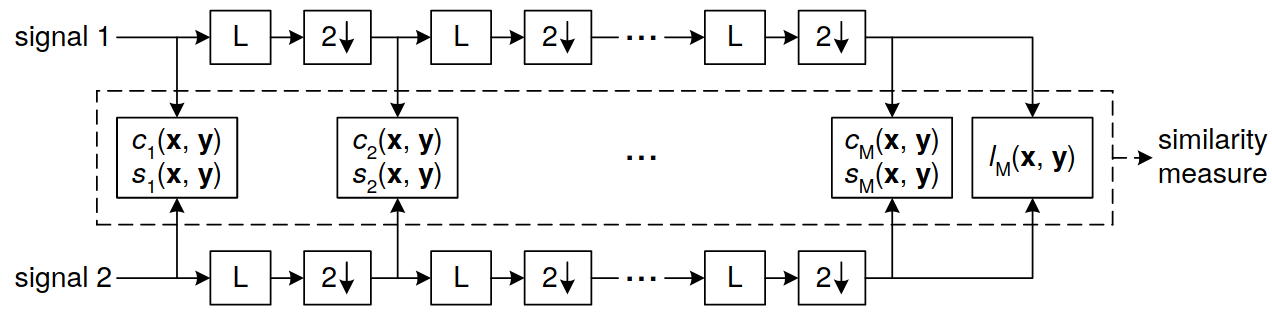
\includegraphics[width=\textwidth]{pic/MS-SSIM}
	\caption{Multi-scale SSIM system, L: lowpass filter, 2$\downarrow$: downsampling by 2 (image source: \cite{1292216})}
	\label{fig:ms_ssim}
\end{figure*}

\begin{displaymath}
	\mathrm{MS\mbox{-}SSIM}(x,y) = I_M(x,y)^{\alpha_M} \prod_{j=1}^{M} C_j(x,y)^{\beta_j}S_j(X,y)^{\gamma_j}
\end{displaymath}

Obviously, the goal is for the network to learn to produce visually pleasing images. To the root of the MS-SSIM is the simple SSIM function. Where for pixel p is defined as 

\begin{equation}
\begin{aligned}
\mathrm{SSIM}(p) &= \frac{2\mu_x\mu_y + C_1}{\mu_x^2 + \mu_y^2 + C_1}\cdot\frac{2\sigma_{xy} + C_2}{\sigma_x^2 + \sigma_y^2 + C_2} \\ 
&= l(p)\cdot cs(p)
\end{aligned}
\end{equation}

Means ($\mu$) and standard deviations ($\sigma$) are computed with a Gaussian filter with standard deviation $\sigma_G$. The max output of this metrics is 1 when the two inputs are similar to each other and the minimum is 0 when they are not. In the training loop we can use the loss function like this:

\begin{equation}
	\mathcal{L}^{\mathrm{SSIM}}(P) = \frac{1}{N}\sum_{p \in P}1-\mathrm{SSIM}(p)
\end{equation}

where the p is the pixel and we are looking at its neighborhood as large as the support of the G ($\sigma_G$). So, we can write the loss as

\begin{equation}
\mathcal{L}^{\mathrm{SSIM}}(P) = 1-\mathrm{SSIM}(\tilde{p})
\end{equation}

because the convolutional nature of the network, where the $\tilde{p}$ is the center pixel of patch P. 
The processed quality depends on the size of $\sigma_G$, but rather then fine-tuning it we can use MS-SSIM. Further information you can visit the cited source of Nvidia Resource \cite{zhao2015loss}.

\begin{equation}
		\mathrm{MS\mbox{-}SSIM}(p) = l_M^\alpha \cdot \prod_{j=1}^{M}cs_j^{\beta_j}(p)
\end{equation}

% This is here because this way it will be on the top of the correct page
\begin{figure*}[b]
	\centering
	\includegraphics[width=\textwidth]{pic/hyperparamopt}
	\caption{Series of hyperparameter runs}
	\label{fig:hyperparamteres}
\end{figure*}

\section{Hyperparameter optimization}

During development we experimented with multiple architectures and made several extensions to existing implementations, hence our hyperparameter optimization sessions are distributed and made between architectural changes.

% if have a single appendix:
%\appendix[Proof of the Zonklar Equations]
% or
%\appendix  % for no appendix heading
% do not use \section anymore after \appendix, only \section*
% is possibly needed

% use appendices with more than one appendix
% then use \section to start each appendix
% you must declare a \section before using any
% \subsection or using \label (\appendices by itself
% starts a section numbered zero.)
%

%\appendices
\section{The whole development process}
%\label{appendix:development}

\subsection{InfoGAN-based models}

At first, to get familiar with the problem we tried to solve we started the development process with examining the original InfoGAN paper and existing implementations. Our first network was a simple InfoGAN implementation based on these sources \cite{chen2016infogan}. To start from a simple problem we generated MNIST-like images. The results were promising, because we successfully reproduced the results presented in the InfoGAN paper for MNIST.

\begin{figure}[h!]
	\centering
	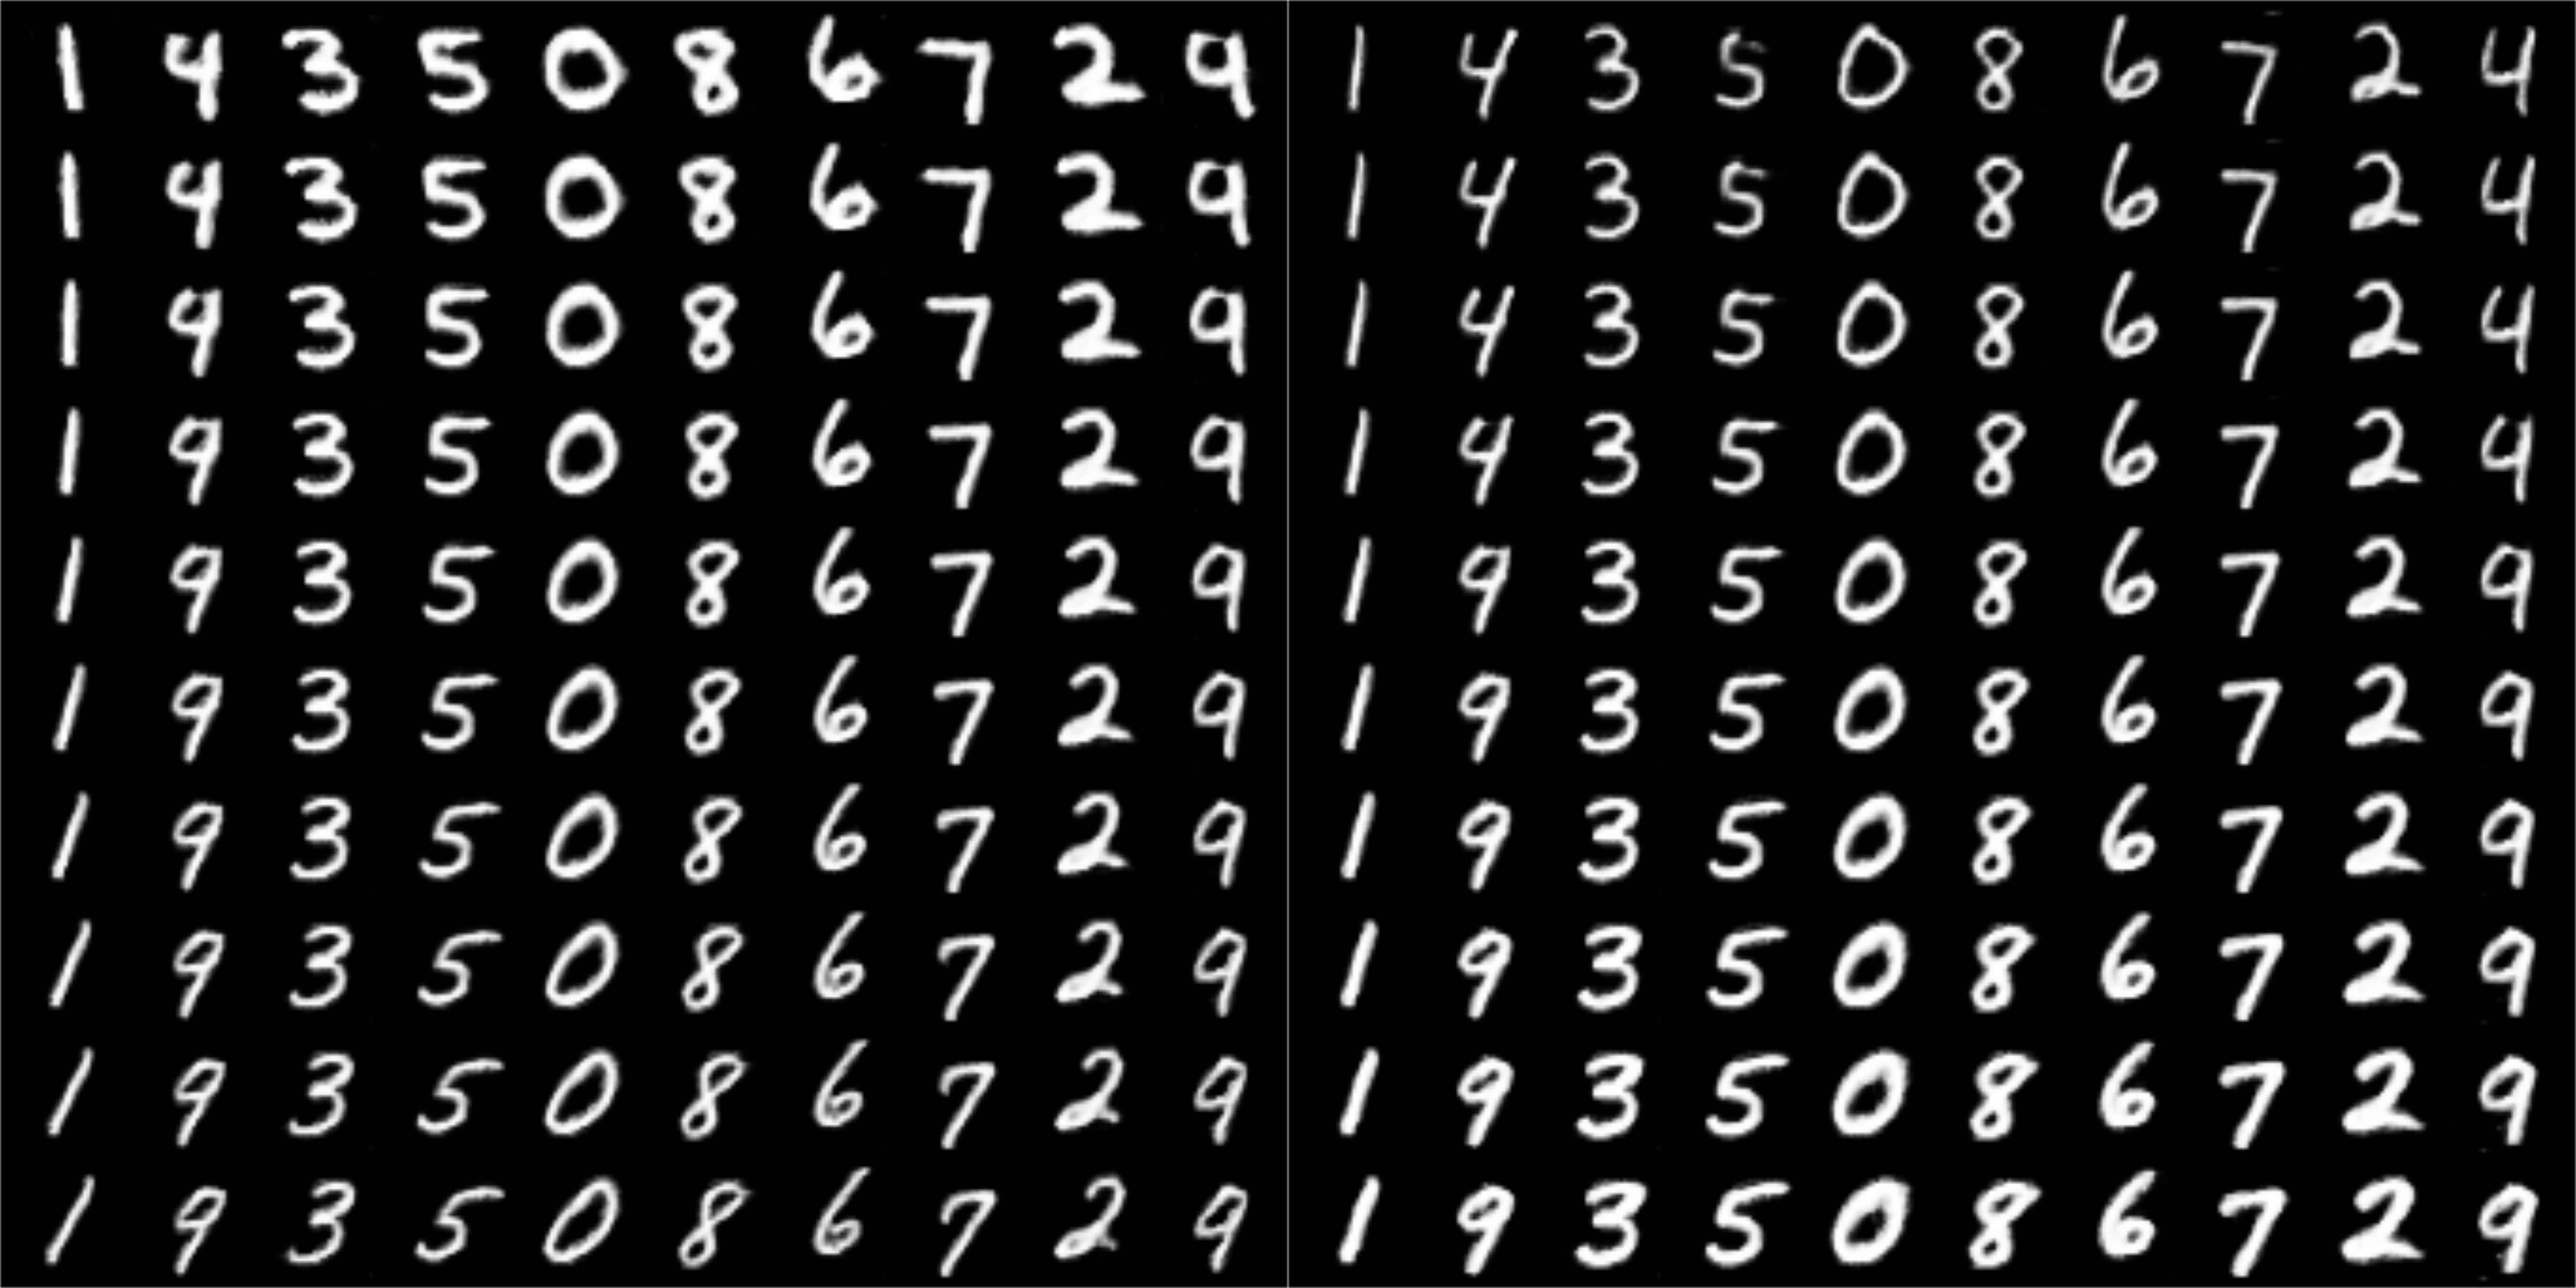
\includegraphics[width=1\linewidth]{pic/mnist}
	\caption{First feature-controlled generation for handwritten digits. Each column corresponds to one state of the categorical code component, controlling which digit is being generated. On the left, $c_1$ continuous component varies controlling the angle of the written digits, while at the right, $c_2$ varies controlling the thickness of the digits.}
	\label{fig:mnist_results}
\end{figure}

The next step was to switch dataset and to try to generate controlled images of celebrities. We started with a picture size of 64x64 pixel and managed to generate mid-quality images.

\begin{figure}[h]
	\centering
	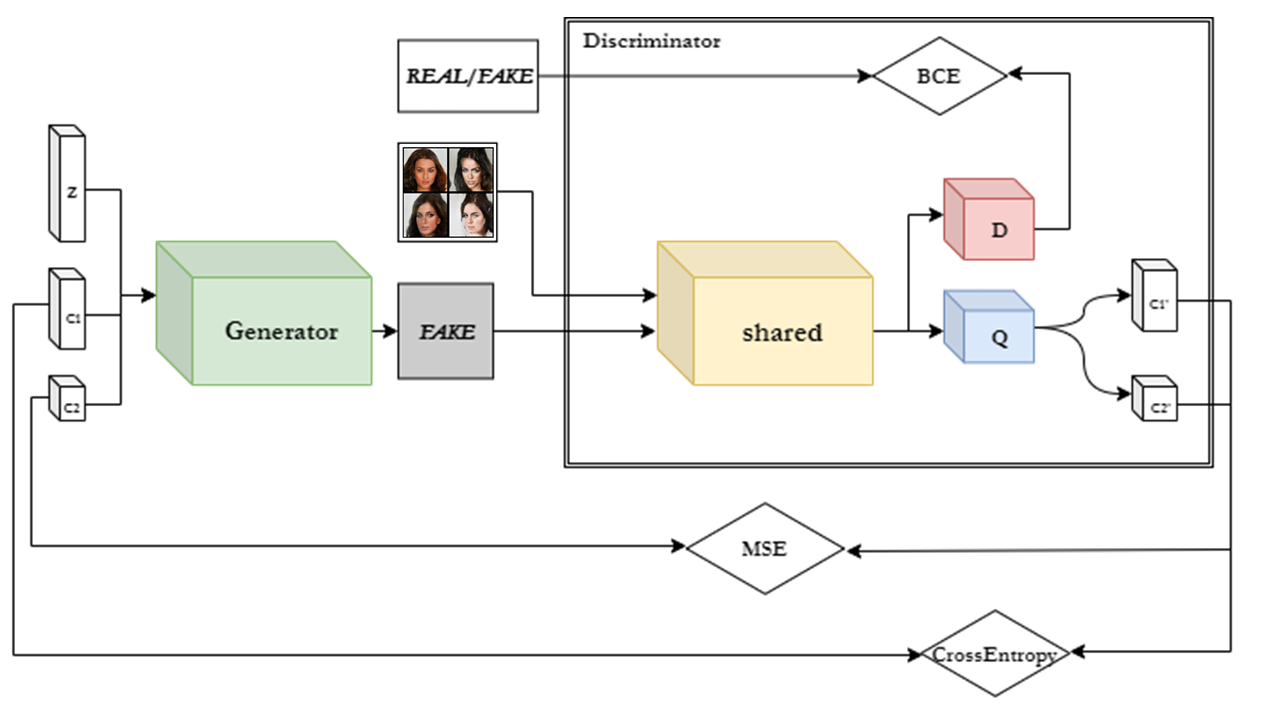
\includegraphics[width=\linewidth]{pic/1}
	\caption{First InfoGAN implementation}
	\label{fig:infogan}
\end{figure}




\subsubsection{Extending InfoGAN with noise-vector recovery}

The InfoGAN implementation we based our work on implements the code recovery and discriminator with the use of a shared network: it comprises of the convolutional layers that process the real and fake images, and the code recovery as well as the decision making (discriminator functionality) comes after this common part.

\begin{figure}[h]
	\centering
	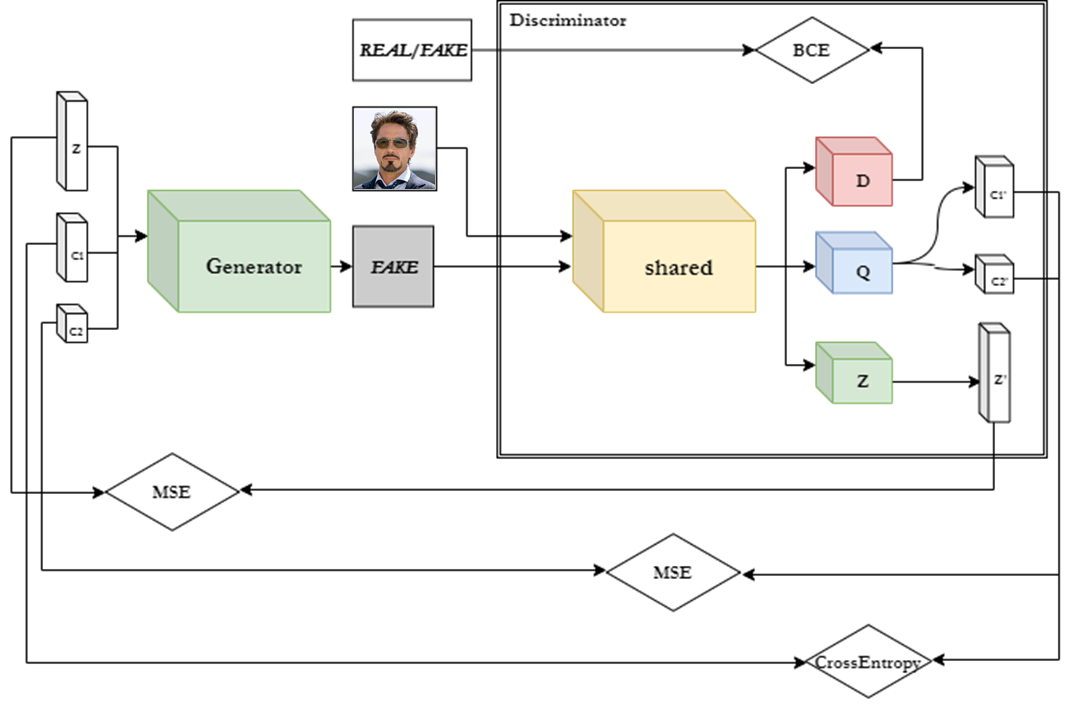
\includegraphics[width=\linewidth]{pic/Infogan_diss_predicting}
	\caption{Extended InfoGAN implementation}
	\label{fig:infogan_simple_noise}
\end{figure}



Because our goal was to alter existing images with our network, the first extension we added to the original InfoGAN was a noise-recovering FC-layer after the shared network, similar to the one used for code recovery. We defined the same L2-loss for this noise predictor just like we did for code recovery, and simply added it to the total info-loss with a 0.1 coefficient.

\begin{figure}[h]
	\centering
	\includegraphics[width=\linewidth]{pic/tony_regen}
	\caption{First image regeneration results}
	\label{fig:tony_regen}
\end{figure}


\subsubsection{Suppressing the discriminator with added noise}

After multiple training sessions with the extended InfoGAN we realized that at the beginning of the training the discriminator gains too much advantage. The loss of the generator starts from a high value and decreases slowly because it cannot compete with the discriminator.

To disrupt the discriminator we added Gaussian noise to its input. By controlling the power of the added noise we can suppress the discriminator to make room for improvement of the generator.

\begin{figure}[h]
	\centering
	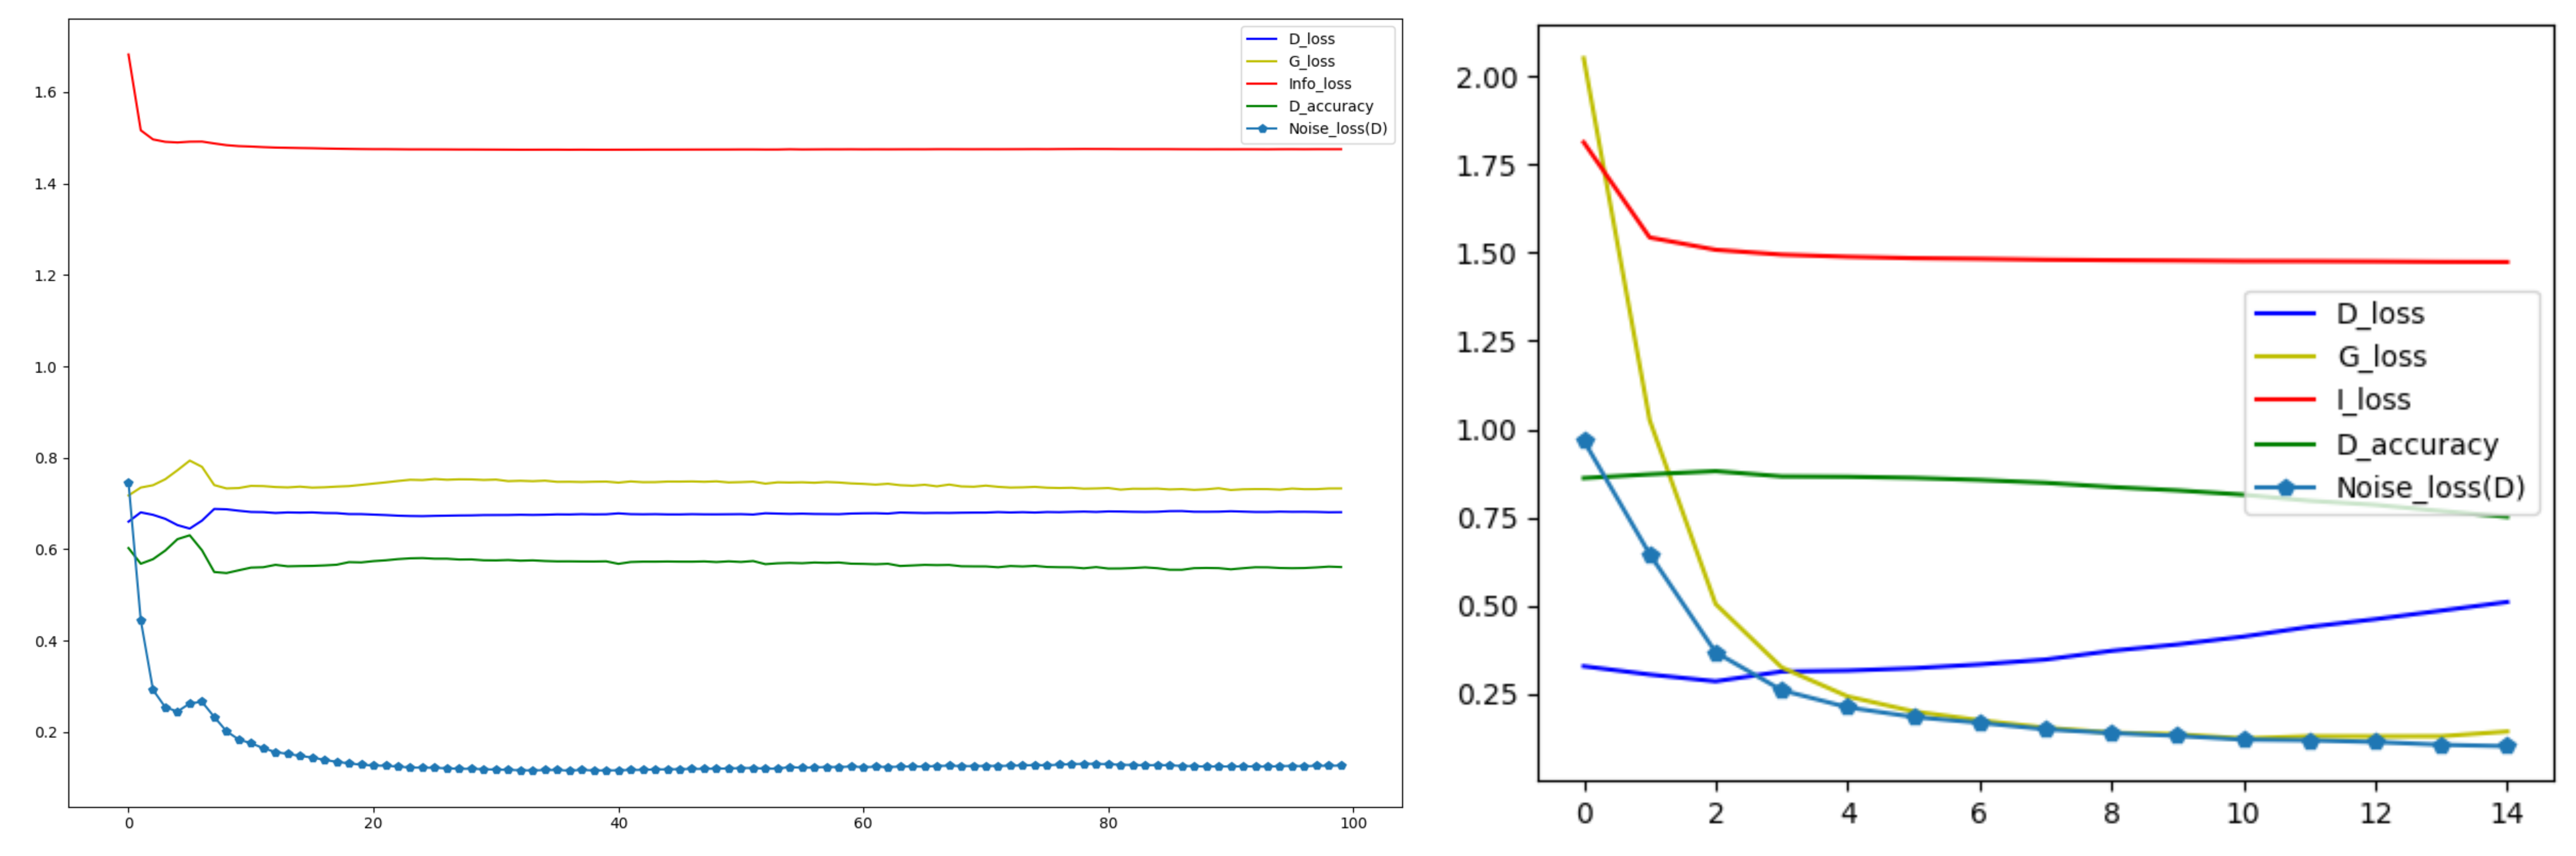
\includegraphics[width=\linewidth]{pic/added_noise}
	\caption{Improved convergence with disruptive noise on the discriminator's input}
	\label{fig:added_noise}
\end{figure}

We started our first hyperparameter optimization session at this point. The hyperparameters and their sets of values were the following:

\begin{itemize}
	\item Image size: \{32x32, 64x64\}
	\item Dimension of the latent vector (noise and code concatenated): \{64, 128\}
	\item Dimensions of categorical code: \{8, 10\}
	\item Noise "power": \{1/15, 1/20\}
	\item Learning rate: \{$10^{-4}, 2 \cdot 10^{-4}$\}
	\item Batch size: \{8, 64, 128, 512\}
	\item Epochs: \{15, 20, 42, 50, 100\}
\end{itemize}

As a result of this optimization process we learned that: 1) one learning rate for all subnetworks may not be the best choice, 2) the image size and the size of the latent vector should change together to maintain quality, 3) batch size largely effects the quality of the generated images, 4) the higher value of noise power is needed for balanced training.

Another problem was the recovery of the noise part of the latent vector. Convergence of noise recovery slowed down then stalled in a state that did not provide sufficient image recovery.

%\begin{figure*}[t]
%	\centering
%	\includegraphics[width=\textwidth]{hyperparamopt}
%	\caption{Series of hyperparameter runs}
%	\label{fig:hyperparamteres}
%\end{figure*}

\subsubsection{Separating the discriminator from latent vector recovery network}

After we extended the original InfoGAN architecture and run multiple training sessions we decided to separate the discriminator from the latent vector predictor. We hypothesized that the shared layers cannot be optimized if they had to adapt according to three different objectives and loss functions.

\begin{figure}[h]
	\centering
	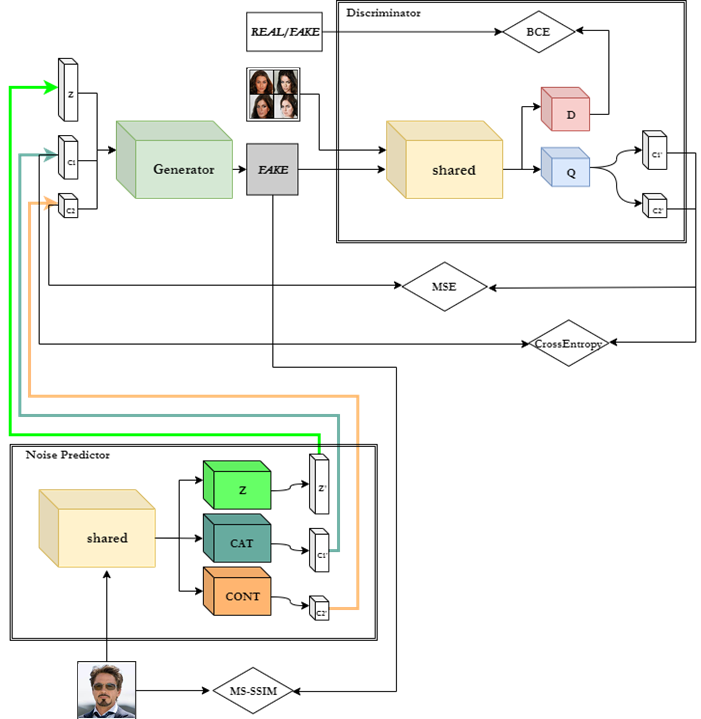
\includegraphics[width=\linewidth]{pic/2}
	\caption{Extended InfoGAN implementation with separate predictor network}
	\label{fig:infogan_noise}
\end{figure}

First, we removed the noise recovery layer and created a new, independent network. This way only two task remained for the discriminator: making a decision about the input image (real or fake) and to recover its control code components (for mutual information maximization).

The next step was to extend the predictor network to predict the whole latent vector of real images that are desired to be altered. The resulting architecture can be seen in Fig. \ref{fig:infogan_noise}. This extended predictor network should become, in theory, the inverse of the generator, effectively forming an autoencoder with it.

Results became better with a slightly faster convergence. To further improve the performance of noise recovery we experimented with some of the hyperparameters, then tried to approximate the practical limit of noise recovery (see below).

\subsubsection{Iterative noise recovery}

To find the limit of the noise recovery to a given generator we tried to iteratively approximate the noise vector. The quality of the recovery highly depends on the resolution of the generated images by the generator. 

\begin{figure}[h]
	\centering
	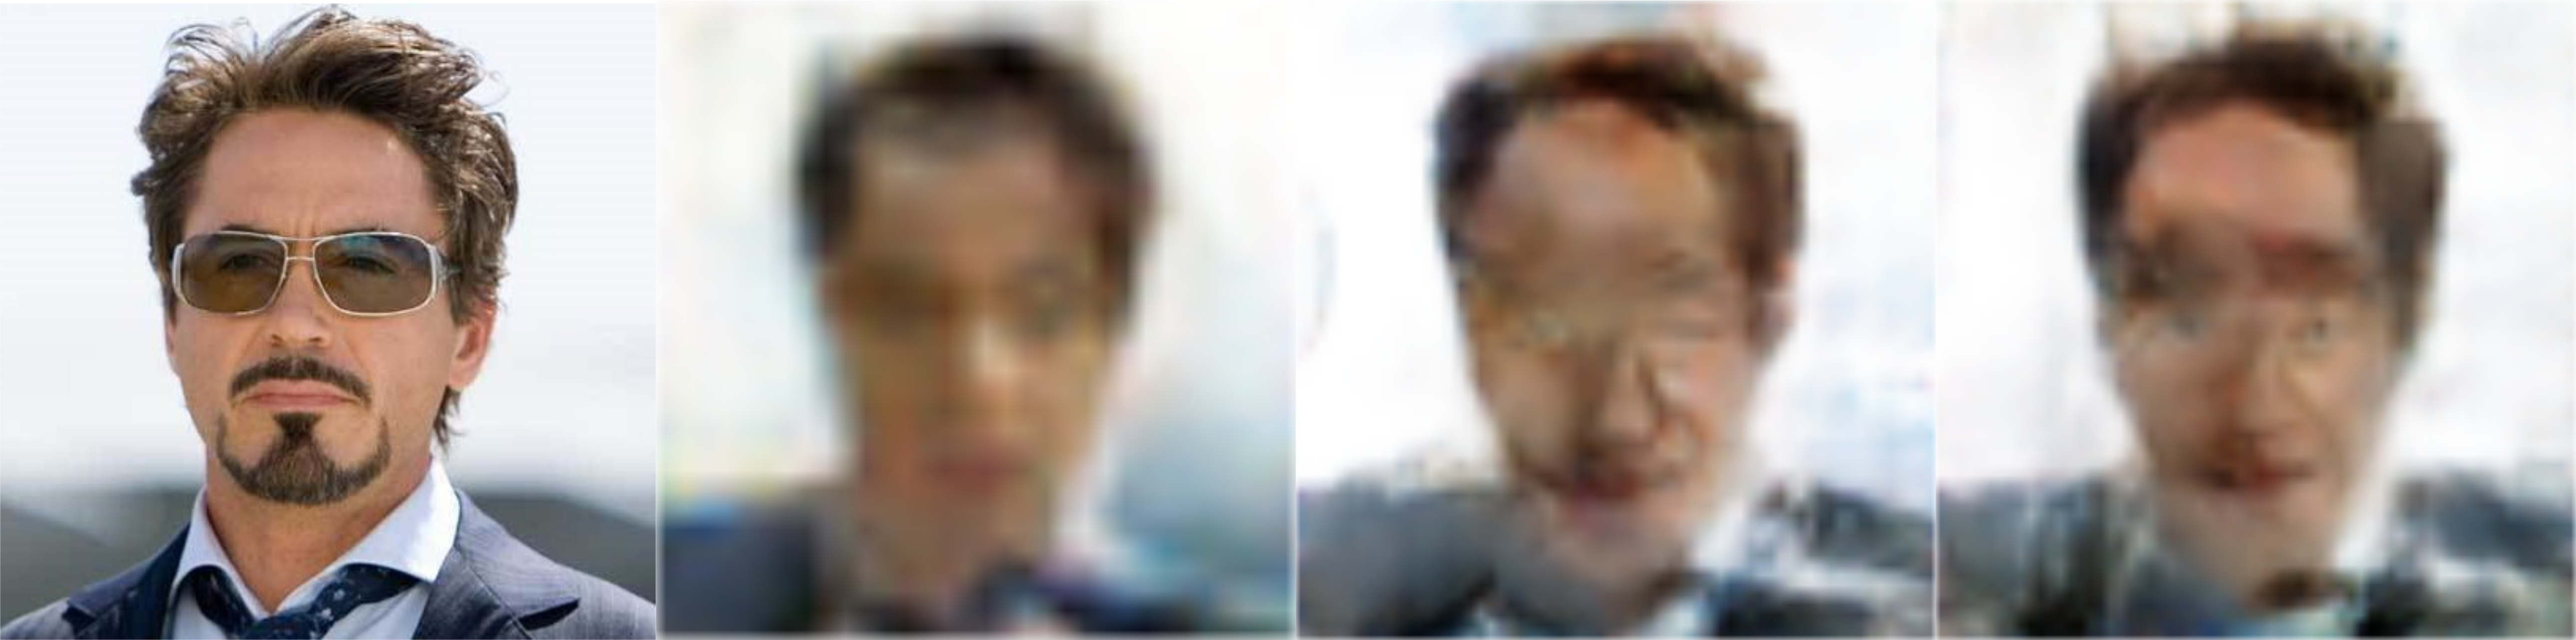
\includegraphics[width=\linewidth]{pic/tony_iterative}
	\caption{Results of iterative noise approximations with different error functions (from left to right): original image, MSE, SSIM, MS-SSIM}
	\label{fig:tony_iterative}
\end{figure}

We tried to fine-tune the latent vector with a generator trained on 32x32 images and 64x64 ones and the latter one proves the theory. We used only the Generator and an Adam optimizer to fine-tune the latent vector. Our goal was to get the appropriate vectors which we can feed to the generator for the desired image generation. We found out that the limit is not yet reached with the noise predictor but the generator is also a limiting factor in the recovery process, hence we started to look for ideas to improve image quality.

\begin{figure}[b]
	\centering
	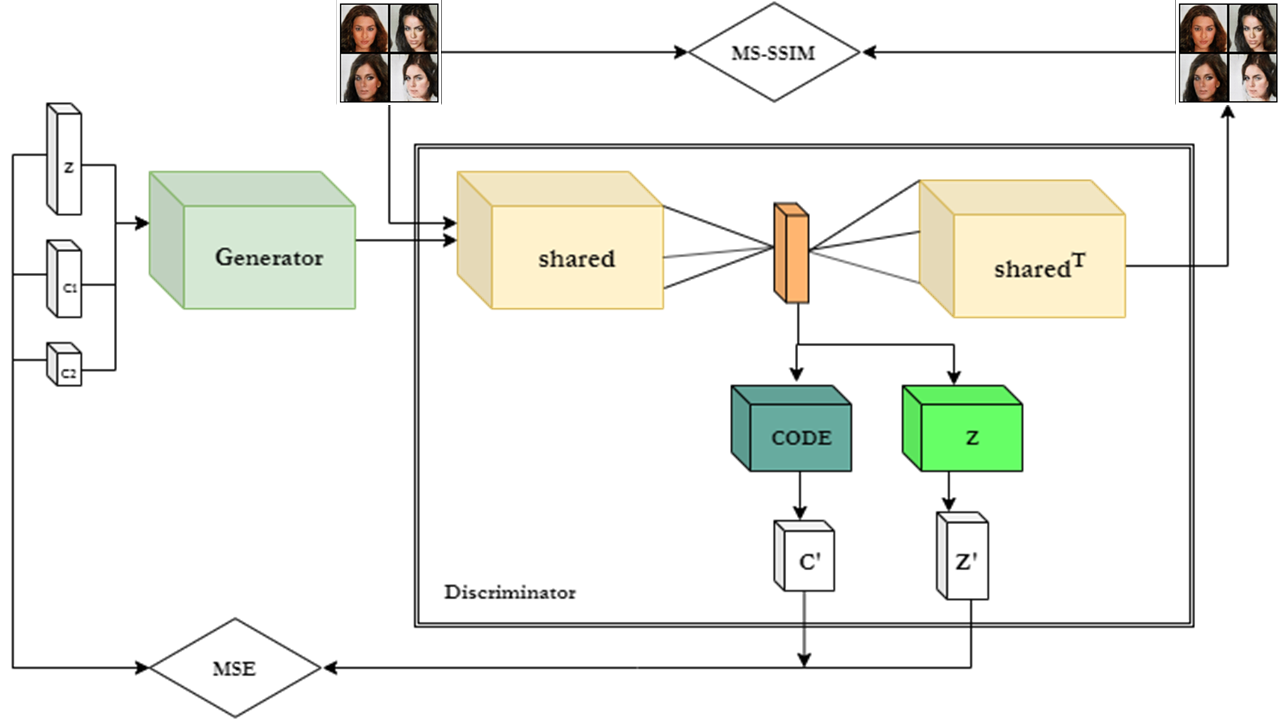
\includegraphics[width=\linewidth]{pic/3}
	\caption{Architecture using autoencoder as discriminator (BEGAN-inspired)}
	\label{fig:infogan_ae}
\end{figure}

\subsection{InfoGAN-BEGAN hybrids}

After several attempts to improve image quality of the modified InfoGAN architecture we looked for new architectural ideas. The search ended with the Boundary Equilibrium GAN and the idea of implementing the discriminator as an autoencoder. We examined and merged this idea into our network.

\subsubsection{Using an Autoencoder as discriminator}

Borrowing the idea from the BEGAN architecture we modified our discriminator to form an autoencoder. We used the layers of discriminator for image encoding, and the layers of the generator for decoding.

Unfortunately, the structure of the previously used subnetworks proved to be suboptimal to form an autoencoder. We tried to make their structure more symmetrical but eventually reached the conclusion that we have to implement the discriminator from scratch.

\subsubsection{Implementing BEGAN and extending it with noise recovery}

After the effectively failed attempt of tailoring the InfoGAN architecture to be more like BEGAN, we tried the other direction: implementing BEGAN and modifying it to meet our goals. We extended an existing implementation with our previously developed predictor network, the resulting architecture can be seen on Fig. \ref{fig:infogan_ae_noise}.

\begin{figure}[h]
	\centering
	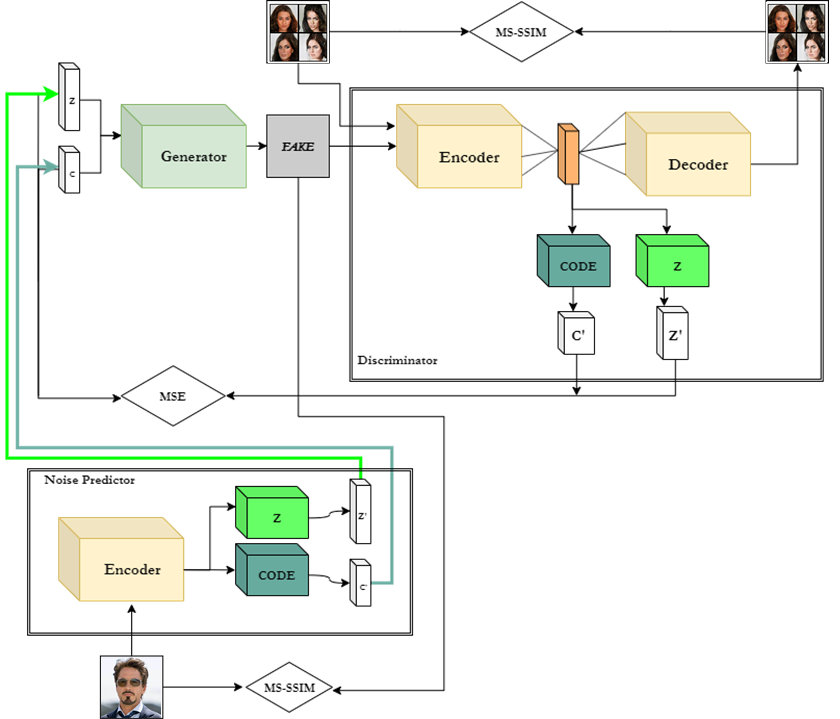
\includegraphics[width=\linewidth]{pic/BInfoGAN+predictor}
	\caption{Architecture using autoencoder as discriminator (BEGAN-inspired) extended with noise predictor network}
	\label{fig:infogan_ae_noise}
\end{figure}

The generated images had better quality than before but we could not control their properties. We conducted multiple experiments with this network and eventually found out that the base BEGAN implementation suffers from mode collapse with the given set of hyperparameters.

\subsubsection{Improving image quality with advanced loss functions}

To improve the quality of generated images we looked for advanced loss functions to find more meaningful metrics than MSE.

The first candidate was Structural Similarity (SSIM) method. This metric was developed to approximate human perception of image quality and comprises of three components: luminance, contrast and structure. This method is used extensively for iterative latent code approximation and it proved to be better than MSE for our purposes.

To further improve the image quality, especially when generating 128x128 pixel images, we used the Multi-scale Structural Similarity method (Fig. \ref{fig:ms_ssim}).

We also used these functions to iteratively approximate the to-be-predicted noise vector and the limit of recovery.

\subsection{Improving image quality of Info-BEGAN with VGG-based image embedding}

After we experimented with multiple quality improving methods we found a new and promising one: instead of comparing the original and recovered images pixel-by-pixel we can embed them into a feature space and compute their distance in that space.

To implement this kind of image comparison multiple source \cite{abdal2019image2stylegan} uses the first few layers of the VGG-16 image classification network because these convolutional layers can detect low-to-mid level image features and can create a meaningful latent space.

We modified our image evaluation method to first make this embedding then compute L2-distance between the resulting vectors. We used the first 23 layers of the feature extractor part, then flattened the 14x14x512 sized output.

This idea of using image embedding to determine a meaningful distance metric for images needs further development because we see great potential in it but had no time to complete the integration of it.

% you can choose not to have a title for an appendix
% if you want by leaving the argument blank
%\section{}
%Appendix two text goes here.

\section{Results}
The results were not as satisfying as we wanted. It seems the InfoGAN architecture is focused only on the maximization of the mutual information and not to produce visually pleasing images. We also noticed, that for a good prediction the Noise Predictor needs to have a Generator that can produce images with good quality. Also, the resolution is important, because we tried both 64x64 and 128x128 images, and the bigger resolution led to better quality of reconstruction. At this area we had to handle a trade-off because the better-quality demand much more compute performance or much more training time. We trained our model with a Nvidia TitanX P with 12GB GPU memory. We completed more than 30 training and several of them was over 30 hours.

\begin{figure}[h]
	\centering
	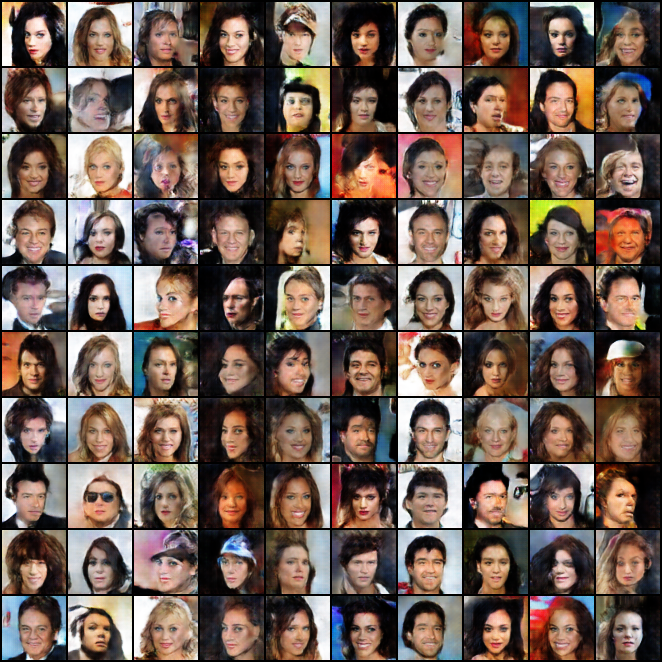
\includegraphics[width=1\linewidth]{pic/best1}
	\caption{Best results of our InfoGAN-based architecture}
	\label{fig:best1}
\end{figure}

\begin{figure}[h]
	\centering
	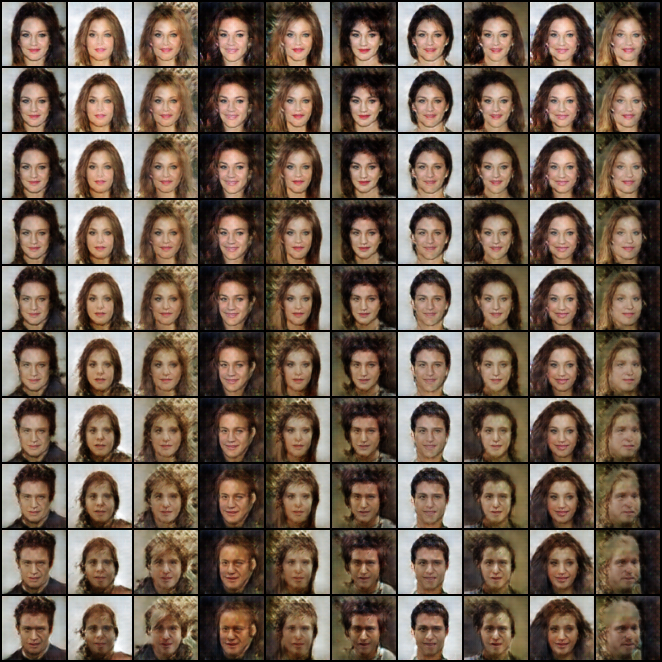
\includegraphics[width=1\linewidth]{pic/best2}
	\caption{Controlled image generation with InfoBEGAN and noise predictor}
	\label{fig:best2}
\end{figure}

\begin{figure}[h]
	\centering
	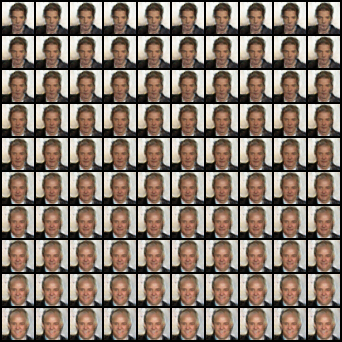
\includegraphics[width=1\linewidth]{pic/predict_everything}
	\caption{Best results of InfoGAN architecture with separated noise predictor}
	\label{fig:best3}
\end{figure}

On our results obviously visible the bad generation and quality caused fault. Some part of the result pictures contains the information what we want, but overall the generated images are not usable for data augmentation yet.

\section{Future plans}
To improve the generation quality, we will try to further develop the Info-BEGAN architecture and continue experimenting with image embedding. Further hyperparameter optimization is also considered due to lack of time to optimize the latest architecture. We hope we can develop a highly controllable generator on the foundation laid by these extensive experiments conducted during this semester.


% use section* for acknowledgment
\ifCLASSOPTIONcompsoc
  % The Computer Society usually uses the plural form
  \section*{Acknowledgments}
\else
  % regular IEEE prefers the singular form
  \section*{Acknowledgment}
\fi


We would like to thank Márton Szemenyei, Lecturer from the Department of Control Engineering and Information Technology, for his endless help and guidance during the semester.


% Can use something like this to put references on a page
% by themselves when using endfloat and the captionsoff option.
\ifCLASSOPTIONcaptionsoff
  \newpage
\fi



% trigger a \newpage just before the given reference
% number - used to balance the columns on the last page
% adjust value as needed - may need to be readjusted if
% the document is modified later
%\IEEEtriggeratref{8}
% The "triggered" command can be changed if desired:
%\IEEEtriggercmd{\enlargethispage{-5in}}

% references section

% can use a bibliography generated by BibTeX as a .bbl file
% BibTeX documentation can be easily obtained at:
% http://mirror.ctan.org/biblio/bibtex/contrib/doc/
% The IEEEtran BibTeX style support page is at:
% http://www.michaelshell.org/tex/ieeetran/bibtex/
%\bibliographystyle{IEEEtran}
% argument is your BibTeX string definitions and bibliography database(s)
%\bibliography{IEEEabrv,../bib/paper}
%
% <OR> manually copy in the resultant .bbl file
% set second argument of \begin to the number of references
% (used to reserve space for the reference number labels box)
%\begin{thebibliography}{1}

%\bibitem{IEEEhowto:kopka}
%H.~Kopka and P.~W. Daly, \emph{A Guide to {\LaTeX}}, 3rd~ed.\hskip 1em plus
%  0.5em minus 0.4em\relax Harlow, England: Addison-Wesley, 1999.



%\end{thebibliography}

%\include{citation}
%\bibliographystyle{IEEEtr}

\bibliographystyle{IEEEtran}
%\clearpage
\bibliography{citation}

% biography section
% 
% If you have an EPS/PDF photo (graphicx package needed) extra braces are
% needed around the contents of the optional argument to biography to prevent
% the LaTeX parser from getting confused when it sees the complicated
% \includegraphics command within an optional argument. (You could create
% your own custom macro containing the \includegraphics command to make things
% simpler here.)
%\begin{IEEEbiography}[{\includegraphics[width=1in,height=1.25in,clip,keepaspectratio]{mshell}}]{Michael Shell}
% or if you just want to reserve a space for a photo:

%\begin{IEEEbiography}{Michael Shell}
%Biography text here.
%\end{IEEEbiography}

% if you will not have a photo at all:
%\begin{IEEEbiographynophoto}{John Doe}
%Biography text here.
%\end{IEEEbiographynophoto}

% insert where needed to balance the two columns on the last page with
% biographies
%\newpage

%\begin{IEEEbiographynophoto}{Jane Doe}
%Biography text here.
%\end{IEEEbiographynophoto}

% You can push biographies down or up by placing
% a \vfill before or after them. The appropriate
% use of \vfill depends on what kind of text is
% on the last page and whether or not the columns
% are being equalized.

%\vfill

% Can be used to pull up biographies so that the bottom of the last one
% is flush with the other column.
%\enlargethispage{-5in}



% that's all folks
\end{document}


